% Autor szablonu: dr Roman Czapla
% Kompilacja: pdfLaTeX (dwukrotnie, aby zaktualizować spis treści).
% Wymagane logo uczelni: images/logo.png (ścieżka względem pliku głównego).
\documentclass[11pt,a4paper,oneside]{article}
\usepackage[utf8]{inputenc}
\usepackage[T1]{fontenc}
\usepackage[polish,provide=*]{babel}
\usepackage{lmodern,microtype}
\usepackage[margin=25mm,headheight=14pt]{geometry}
\usepackage{xcolor,graphicx,tabularx,booktabs,array,enumitem,fancyhdr,titlesec}
\usepackage[hidelinks]{hyperref}
\usepackage{tikz}
\usetikzlibrary{positioning,arrows.meta}
\usepackage{xurl}
\definecolor{accent}{HTML}{344B59}
\definecolor{hintcolor}{HTML}{58636A}
\hypersetup{pdfauthor={Wojciech Czachurski, Julia Gawlik, Dawid Pątko},pdftitle={Projekt inżynierski -- Dokumentacja projektowa}}
\setlength{\parindent}{0pt}
\setlength{\parskip}{6pt}
\renewcommand{\arraystretch}{1.3}
\setlength{\emergencystretch}{2em}
\setlist[itemize]{leftmargin=*,itemsep=2pt,topsep=3pt}
\titleformat{\section}{\Large\bfseries\color{accent}}{\thesection.}{0.5em}{}
\titleformat{\subsection}{\large\bfseries\color{accent}}{\thesubsection.}{0.5em}{}
\pagestyle{fancy}
\fancyhf{}
\fancyhead[L]{\small Projekt inżynierski}
\fancyhead[R]{\small Dokumentacja projektowa}
\fancyfoot[C]{\small\thepage}
\renewcommand{\headrulewidth}{0.3pt}
\newcolumntype{Y}{>{\raggedright\arraybackslash}X}

% Podpowiedzi są widoczne podczas wypełniania szablonu.
% Przed oddaniem: uzupełnij pola, zastąp przykłady własną treścią
% i zmień poniższy przełącznik na \podpowiedzifalse.
\newif\ifpodpowiedzi
%\podpowiedzitrue
\podpowiedzifalse
\newcommand{\podpowiedz}[1]{\ifpodpowiedzi\par\begingroup\small\color{hintcolor}\textit{Wskazówka: #1}\par\endgroup\fi}
\newcommand{\pole}[1]{\textnormal{[#1]}}

% Dane dokumentu -- uzupełnij w jednym miejscu.
% Ścieżkę logo można zmienić poniżej.
\newcommand{\pliklogo}{images/logo.png}
\newcommand{\logouczelni}{%
  \includegraphics[width=0.8\textwidth,height=40mm,keepaspectratio]{\pliklogo}%
}
\newcommand{\tytulprojektu}{System do zarządzania rozgrywkami sportowymi}
\newcommand{\rokakademicki}{2026/2027}
\newcommand{\semestrprojektu}{VII, zimowy}
\newcommand{\datadokumentu}{19.11.2026}
\newcommand{\wersjadokumentu}{1.0}
% Zespół dwuosobowy tylko za zgodą dyrekcji: zmień na \trzeciaosobafalse.
\newif\iftrzeciaosoba
\trzeciaosobatrue
\newcommand{\studentA}{Wojciech Czachurski}
\newcommand{\studentB}{Julia Gawlik}
\newcommand{\studentC}{Dawid Pątko}
\newcommand{\albumA}{168750}
\newcommand{\albumB}{168679}
\newcommand{\albumC}{168744}
\newcommand{\prowadzacyA}{mgr Wojciech Baran}
\newcommand{\prowadzacyB}{dr Wojciech Gwizdała}

\begin{document}
\begin{titlepage}
\centering
{\large Uniwersytet Komisji Edukacji Narodowej w Krakowie\par}
{\normalsize Instytut Bezpieczeństwa i Informatyki\par}
\vspace{8mm}
\logouczelni\par
\vspace{10mm}
{\Large\bfseries\color{accent} PROJEKT INŻYNIERSKI\par}
\vspace{3mm}
{\large Dokumentacja projektowa\par}
\vspace{15mm}
{\LARGE\bfseries\tytulprojektu\par}
\vspace{15mm}
{\small ZESPÓŁ PROJEKTOWY\par}
\vspace{3mm}
\begin{tabular}{ll}
\studentA & Nr albumu: \albumA\\
\studentB & Nr albumu: \albumB
\iftrzeciaosoba\\
\studentC & Nr albumu: \albumC\fi
\end{tabular}
\vspace{12mm}

{\small PROWADZĄCY ZAJĘCIA PROJEKTOWE\par}
\vspace{3mm}
\prowadzacyA\par
\prowadzacyB\par
\vfill
Rok akademicki: \rokakademicki\quad Semestr: \semestrprojektu\par
Data dokumentu: \datadokumentu\quad Wersja: \wersjadokumentu\par
\vspace{6mm}
Kraków\par

\end{titlepage}

\tableofcontents
\sloppy
\podpowiedz{Dokument opisuje finalne rozwiązanie i umożliwia zrozumienie jego budowy oraz dalszą pracę nad projektem. Zakres uzgodnij z prowadzącymi: usuń podsekcje nieadekwatne do projektu i dodaj potrzebne. UML, baza danych i opis kodu nie są obowiązkowe dla każdego rodzaju projektu. Opis przebiegu pracy i indywidualnego wkładu należy do sprawozdania końcowego. Uzupełnij pola i wyłącz podpowiedzi przed oddaniem.}

\section{Szczegółowa dokumentacja projektowa}
\subsection{Zakres i identyfikacja rozwiązania}
\podpowiedz{Opisz przeznaczenie projektu, najważniejsze wymagania oraz wersję, której dotyczy dokumentacja. Wskaż, gdzie znajdują się pliki źródłowe i zasoby: repozytorium dla projektu programistycznego lub inne miejsce uzgodnione z prowadzącymi. Podaj commit, tag albo oznaczenie wersji plików.}
\textbf{Przeznaczenie i zakres:} aplikacja webowa do organizacji i prowadzenia amatorskich rozgrywek sportowych. Organizator w panelu zakłada turniej w jednym z trzech formatów -- liga (każdy z każdym), puchar (pojedyncza eliminacja) albo grupy z fazą pucharową -- w jednym z trzech sportów: piłka nożna, koszykówka, siatkówka. Dodaje drużyny, zawodników i obiekty, generuje terminarz lub drabinkę, wpisuje wyniki, przebieg meczu na żywo i zdarzenia meczowe, rozpatruje zgłoszenia drużyn i tworzy grafiki do mediów społecznościowych. Tabela i klasyfikacja zawodników są liczone przez system. Kibice oglądają turniej na publicznej stronie pod adresem \texttt{/t/\{slug\}}. Dodatkowo lokalny serwer MCP pozwala prowadzić turniej asystentowi AI w aplikacji Claude Desktop.\par
\textbf{Wersja projektu:} wersja 1.0, gałąź \texttt{main} repozytorium, stan z 19.11.2026.\par
\textbf{Materiały źródłowe:} repozytorium \url{https://github.com/dawer2253/sports-tournament-app} (monorepo). Dokumentacja techniczna dla programistów leży w repozytorium: \texttt{README.md}, \texttt{AGENTS.md}, \texttt{CONTEXT.md} (słownik pojęć domeny), katalog \texttt{docs/} (plan i decyzje projektowe w \texttt{docs/PLAN.md}, rekordy decyzji architektonicznych w \texttt{docs/adr/}, uruchamianie backendu w \texttt{docs/BACKEND.md}, serwer MCP w \texttt{docs/MCP.md}).

\newpage
\subsection{Architektura i organizacja projektu}
\podpowiedz{Przedstaw główne elementy rozwiązania, ich odpowiedzialności i powiązania. Dla aplikacji opisz komponenty i przepływ danych; dla animacji 3D -- organizację scen, obiektów, zasobów i etapów przetwarzania. Wyjaśnij najważniejsze decyzje i zależności. Dodaj schemat, jeśli pomaga zrozumieć rozwiązanie.}
Rozwiązanie jest zbudowane z niezależnego backendu udostępniającego REST API oraz dwóch aplikacji frontendowych typu SPA (rys.~\ref{fig:architektura}). Wszystkie części leżą w jednym repozytorium (monorepo z przestrzeniami roboczymi npm):

\begin{tabularx}{\textwidth}{@{}p{0.3\textwidth} Y@{}}
\toprule
Katalog & Zawartość i odpowiedzialność\\
\midrule
\texttt{packages/api-contract} & kontrakt API w formacie OpenAPI (\texttt{openapi.yaml}) -- jedyne źródło prawdy o kształcie API; z niego działa też serwer mock (Prism)\\
\texttt{packages/api-client} & typy i klient TypeScript generowane z kontraktu\\
\texttt{packages/ui} & design system: komponenty, motyw, ekrany w Storybooku\\
\texttt{apps/admin} & panel organizatora (React, logowanie), port 5173\\
\texttt{apps/public} & publiczna strona turnieju (React, bez logowania), port 5174\\
\texttt{apps/mcp-server} & lokalny serwer MCP dla asystenta AI\\
\texttt{backend} & Laravel 13: REST API \texttt{/api/v1}, logika rozgrywek, baza MySQL\\
\texttt{e2e} & testy end-to-end (Playwright) przez panel, stronę publiczną i backend\\
\bottomrule
\end{tabularx}

\begin{figure}[htbp]
\centering
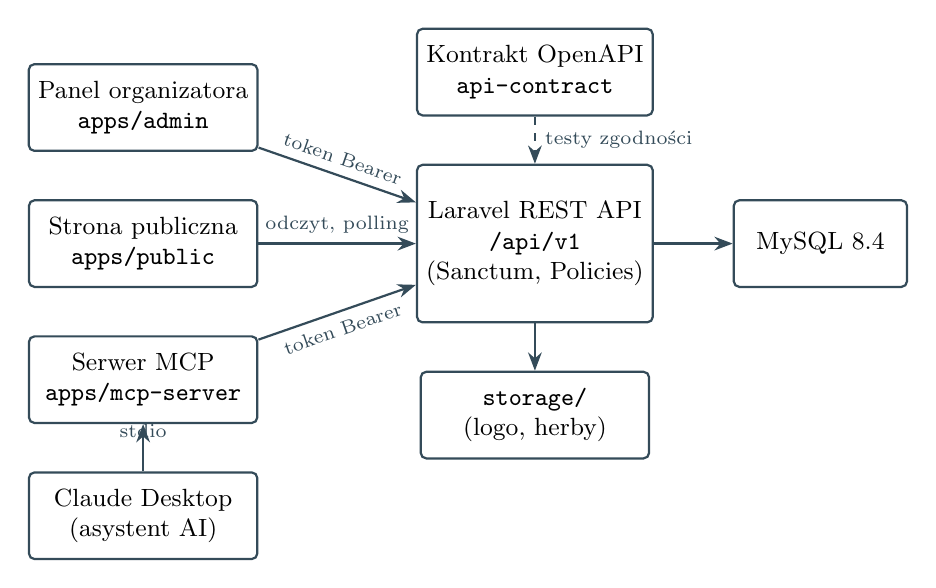
\begin{tikzpicture}[
  box/.style={draw=accent, thick, rounded corners=2pt, align=center, minimum width=29mm, minimum height=11mm, font=\small},
  arr/.style={-{Stealth}, thick, color=accent}]
\node[box] (admin) {Panel organizatora\\\texttt{apps/admin}};
\node[box, below=6mm of admin] (public) {Strona publiczna\\\texttt{apps/public}};
\node[box, below=6mm of public] (mcp) {Serwer MCP\\\texttt{apps/mcp-server}};
\node[box, below=6mm of mcp] (claude) {Claude Desktop\\(asystent AI)};
\node[box, right=20mm of public, minimum height=20mm] (api) {Laravel REST API\\\texttt{/api/v1}\\(Sanctum, Policies)};
\node[box, right=10mm of api, minimum width=22mm] (db) {MySQL 8.4};
\node[box, below=6mm of api] (storage) {\texttt{storage/}\\(logo, herby)};
\node[box, above=6mm of api] (contract) {Kontrakt OpenAPI\\\texttt{api-contract}};
\draw[arr] (admin) -- node[above, font=\scriptsize, sloped]{token Bearer} (api);
\draw[arr] (public) -- node[above, font=\scriptsize]{odczyt, polling} (api);
\draw[arr] (mcp) -- node[below, font=\scriptsize, sloped]{token Bearer} (api);
\draw[arr] (claude) -- node[above, font=\scriptsize]{stdio} (mcp);
\draw[arr] (api) -- (db);
\draw[arr] (api) -- (storage);
\draw[arr, dashed] (contract) -- node[right, font=\scriptsize]{testy zgodności} (api);
\end{tikzpicture}
\caption{Architektura rozwiązania.}
\label{fig:architektura}
\end{figure}

Najważniejsze decyzje architektoniczne:
\begin{itemize}
\item \textbf{Kontrakt przed kodem.} Każda zmiana API zaczyna się od zmiany \texttt{openapi.yaml}, potem regeneruje się klienta TypeScript, a dopiero potem pisze kod. Frontend może pracować na mocku kontraktu, zanim powstanie endpoint, a testy backendu sprawdzają zgodność żądań i odpowiedzi z kontraktem (biblioteka Spectator). CI odrzuca zmianę, w której wygenerowany klient nie odpowiada specyfikacji.
\item \textbf{Dwie osobne aplikacje frontendowe.} Panel wymaga logowania i pozwala edytować dane, strona publiczna tylko je odczytuje. Rozdzielenie upraszcza bezpieczeństwo i pozwala nadać stronie publicznej własny wygląd z kolorem turnieju.
\item \textbf{Jeden korzeń własności.} Organizator (\texttt{User}) jest właścicielem turnieju przez \texttt{Tournament.user\_id}; uprawnienia do drużyn, meczów czy zawodników wynikają z relacji z turniejem (Laravel Policies i zagnieżdżone wiązanie tras).
\item \textbf{Tabela liczona przy odczycie.} Tabela nie jest przechowywana w bazie, tylko liczona z meczów przy każdym żądaniu, dzięki czemu jest zawsze spójna z wynikami.
\item \textbf{Czas w UTC.} API przyjmuje i zwraca daty w UTC z przesunięciem strefy, a przeliczenie na czas lokalny robi frontend.
\item \textbf{Odświeżanie przez polling.} Strona publiczna co 15 sekund (wartość domyślna, \texttt{VITE\_POLL\_INTERVAL\_MS}) ponawia zapytania, a backend odpowiada nagłówkami walidującymi HTTP, więc niezmienione dane nie są przesyłane ponownie.
\end{itemize}
Decyzje są opisane w 14 rekordach ADR w katalogu \texttt{docs/adr/} oraz w dzienniku decyzji w \texttt{docs/PLAN.md}.

\subsection{Modele i diagramy projektowe}
\podpowiedz{Dobierz diagramy do projektu. Dla oprogramowania mogą to być diagramy UML: klas, przypadków użycia, sekwencji, stanów lub komponentów. Dla innych projektów wykorzystaj np. schemat sceny, storyboard lub diagram procesu. Każdy rysunek opatrz podpisem i omów w tekście, stosując odwołania przez \texttt{\textbackslash ref}. Nie twórz diagramów wyłącznie w celu wypełnienia szablonu.}
Rysunek~\ref{fig:model} przedstawia model domeny. Turniej należy do organizatora i ma co najmniej jedną fazę (\texttt{Stage}) -- nawet zwykła liga ma jedną fazę typu \texttt{league}, co pozwala obsłużyć wszystkie formaty jedną ścieżką kodu. Faza grupowa dzieli się na grupy, a każda faza na kolejki lub rundy (\texttt{Round}) zawierające mecze. Drużyny i zawodnicy należą do jednego turnieju.

\begin{figure}[htbp]
\centering
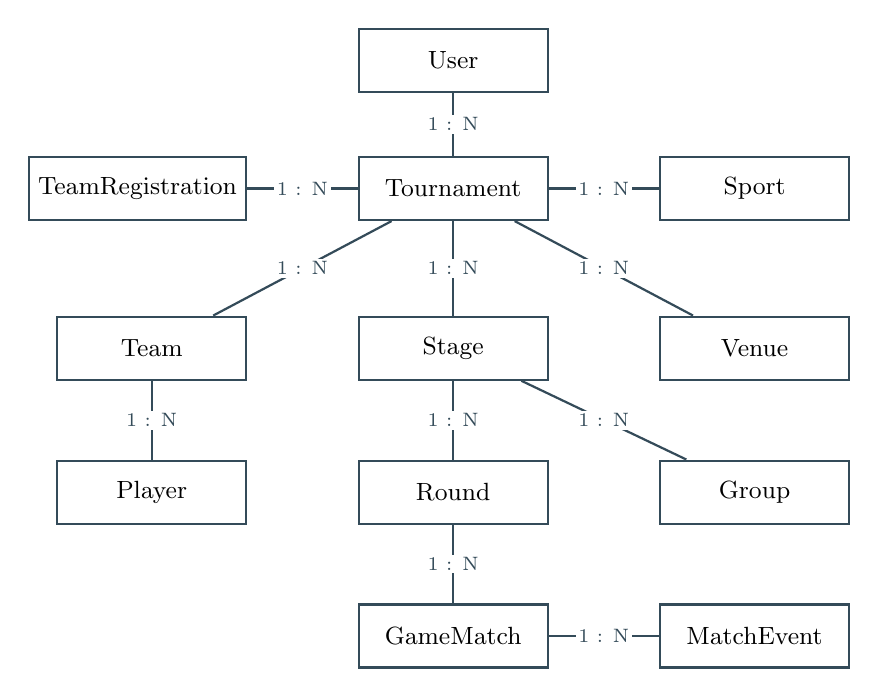
\begin{tikzpicture}[
  ent/.style={draw=accent, thick, align=center, minimum width=24mm, minimum height=8mm, font=\small},
  rel/.style={thick, color=accent},
  lab/.style={font=\scriptsize, fill=white, inner sep=1pt}]
\node[ent] (tour) {Tournament};
\node[ent, above=8mm of tour] (user) {User};
\node[ent, right=14mm of tour] (sport) {Sport};
\node[ent, left=14mm of tour] (reg) {TeamRegistration};
\node[ent, below=12mm of tour] (stage) {Stage};
\node[ent, left=14mm of stage] (team) {Team};
\node[ent, below=10mm of team] (player) {Player};
\node[ent, right=14mm of stage] (venue) {Venue};
\node[ent, below=10mm of stage] (round) {Round};
\node[ent, right=14mm of round] (group) {Group};
\node[ent, below=10mm of round] (match) {GameMatch};
\node[ent, right=14mm of match] (event) {MatchEvent};
\draw[rel] (user) -- node[lab]{1 : N} (tour);
\draw[rel] (sport) -- node[lab]{1 : N} (tour);
\draw[rel] (tour) -- node[lab]{1 : N} (reg);
\draw[rel] (tour) -- node[lab]{1 : N} (stage);
\draw[rel] (tour) -- node[lab]{1 : N} (team);
\draw[rel] (tour) -- node[lab]{1 : N} (venue);
\draw[rel] (team) -- node[lab]{1 : N} (player);
\draw[rel] (stage) -- node[lab]{1 : N} (round);
\draw[rel] (stage) -- node[lab]{1 : N} (group);
\draw[rel] (round) -- node[lab]{1 : N} (match);
\draw[rel] (match) -- node[lab]{1 : N} (event);
\end{tikzpicture}
\caption{Uproszczony model domeny (encje i krotności relacji).}
\label{fig:model}
\end{figure}

Mecz ma cykl życia \texttt{scheduled} $\rightarrow$ \texttt{live} $\rightarrow$ \texttt{finished}. W drabince pucharowej mecz wskazuje, dokąd awansuje zwycięzca (\texttt{winner\_to\_match\_id}) i przegrany (\texttt{loser\_to\_match\_id}, mecz o 3. miejsce). Gdy organizator poprawi wynik i zmieni się zwycięzca, system podmienia drużynę w meczu zależnym, o ile ten jeszcze się nie rozpoczął; jeśli się rozpoczął, zmiana jest blokowana.

Typowy przepływ danych przy wpisaniu wyniku: panel wysyła \texttt{PATCH /matches/\{id\}} z tokenem Bearer; backend sprawdza uprawnienia przez politykę turnieju, waliduje dane w klasie Form Request, zapisuje mecz i ewentualnie przesuwa zwycięzcę w drabince; przy kolejnym odświeżeniu strona publiczna pobiera tabelę, która jest liczona na nowo z meczów zakończonych.

\subsection{Dane, baza danych i zasoby}
\podpowiedz{Jeśli projekt korzysta z bazy danych, opisz schemat, tabele, klucze, relacje, ograniczenia i istotne procedury. Dla innych danych lub zasobów określ formaty, strukturę, pochodzenie oraz sposób przygotowania i wykorzystania. Dla animacji mogą to być modele, tekstury, materiały i pliki dźwiękowe. Wskaż zasoby własne i zewnętrzne oraz warunki ich wykorzystania.}
Baza MySQL 8.4 jest zakładana migracjami Laravela (\texttt{backend/database/migrations}). Najważniejsze tabele:

\begin{tabularx}{\textwidth}{@{}>{\raggedright\arraybackslash}p{0.33\textwidth} Y@{}}
\toprule
Tabela & Zawartość\\
\midrule
\texttt{users} & konta organizatorów; hasła hashowane\\
\texttt{sports} & sporty i ich konfiguracja w kolumnie JSON: domyślna punktacja, typy zdarzeń, dostępne kryteria remisów i statystyki, podział na części meczu lub sety; wiersze wstawiają migracje (dane systemowe)\\
\texttt{tournaments} & turniej: właściciel, sport, unikalny \texttt{slug}, nazwa, logo, kolor, punktacja i kolejność kryteriów remisów (JSON), status \texttt{draft}/\texttt{active}/\texttt{finished}, ustawienia zapisów\\
\texttt{stages}, \texttt{groups}, \texttt{rounds} & struktura turnieju: fazy (\texttt{league}, \texttt{group}, \texttt{knockout}), grupy, kolejki i rundy\\
\texttt{teams}, \texttt{players} & drużyny turnieju (opcjonalnie w grupie) i ich zawodnicy\\
\texttt{venues} & obiekty sportowe turnieju\\
\texttt{matches} & mecze: drużyny, wynik, karne, sety, status, termin, obiekt, krawędzie awansu w drabince\\
\texttt{match\_events} & zdarzenia meczowe (bramka, kartka, rzut za 1/2/3 punkty itp.) z minutą\\
\texttt{team\_registrations} & zgłoszenia drużyn przesłane przez stronę publiczną, oczekujące na decyzję organizatora\\
\texttt{personal\_access\_tokens} & tokeny API wydawane przez Sanctum\\
\bottomrule
\end{tabularx}

Istotne ograniczenia: \texttt{slug} turnieju jest globalnie unikalny, bo buduje publiczny adres; nie można usunąć bytu powiązanego z meczem zakończonym (rozegrany turniej ma pozostać dostępny publicznie); drużyny, zawodnicy i obiekty mają miękkie usuwanie; klucz \texttt{tournaments.user\_id} ma ograniczenie \texttt{RESTRICT}. Kompromisy wynikające z ograniczeń PHP i MySQL opisuje ADR 0005.

Dane demonstracyjne tworzą seedery (\texttt{backend/database/seeders}): sześć turniejów (liga piłkarska, liga koszykówki, liga siatkówki, puchar, grupy z fazą pucharową oraz liga z otwartymi zapisami) z drużynami, zawodnikami, wynikami i zdarzeniami. Komplet tych danych dostają konta organizatorów zespołu oraz domyślne konto demonstracyjne \texttt{administrator@example.com}. Wszystkie nazwy drużyn i zawodników są fikcyjne. Zasoby graficzne (logo aplikacji, ikony, herby zastępcze) są wykonane przez zespół lub pochodzą z bibliotek otwartoźródłowych; fonty Inter, Barlow, Barlow Condensed i Geist są dołączane z pakietów Fontsource i udostępnione na licencji SIL Open Font License.

\subsection{Implementacja i najważniejsze rozwiązania}
\podpowiedz{Dla projektu programistycznego opisz istotne moduły, klasy, funkcje, interfejsy i algorytmy. Podaj znaczenie parametrów, wyniki, ograniczenia i obsługę błędów tam, gdzie jest to potrzebne. Nie wymaga się przepisywania całego kodu ani opisu każdej zmiennej. Dokumentację generowaną z kodu można dołączyć lub wskazać jako osobny materiał.}
\podpowiedz{Dla projektu bez kodu opisz odpowiednie metody wykonania, np. modelowanie, rigging, animację, oświetlenie, rendering i montaż. Podaj istotne ustawienia i uzasadnij ich dobór. Usuń wskazówki nieodnoszące się do projektu.}
\textbf{Warstwa API (backend).} Kontrolery w \texttt{app/Http/Controllers/Api} obsługują zasoby turnieju (turnieje, drużyny, zawodnicy, obiekty, fazy, grupy, mecze, zdarzenia, zgłoszenia, logo) oraz trasy publiczne po \texttt{slug}. Walidację wejścia realizują klasy Form Request, autoryzację -- polityki (\texttt{app/Policies}), a format odpowiedzi -- API Resources. Błędy mają spójny format JSON z komunikatami po polsku; naruszenie reguł domeny (np. edycja meczu zależnego, który już się rozpoczął) kończy się kodem \texttt{422} i niczego nie zapisuje.

\textbf{Generator terminarza} (\texttt{app/Schedule}). \texttt{RoundRobin} układa pary metodą kołową: jedna drużyna stoi w miejscu, pozostałe obracają się o jedną pozycję w każdej kolejce; przy nieparzystej liczbie drużyn dochodzi pauza, która nie jest pokazywana jako mecz. Rewanże odwracają gospodarza. \texttt{DateDistributor} rozkłada kolejki od daty startu co zadany odstęp, a \texttt{CollisionCalculator} przy każdym odczycie terminarza wskazuje kolizje: mecze tej samej drużyny lub na tym samym obiekcie, których okna czasowe (początek plus długość meczu) się nakładają. \texttt{BracketGenerator} i \texttt{BracketSeeding} budują drabinkę pojedynczej eliminacji z wolnymi losami, rozstawieniem ręcznym, losowym albo krzyżowym z grup (1A--2B, 1B--2A).

\textbf{Klasyfikacja} (\texttt{app/Standings}). \texttt{StandingsCalculator} agreguje mecze zakończone fazy lub grupy (mecze, zwycięstwa, remisy, porażki, zdobycze, punkty) i sortuje drużyny według listy kryteriów turnieju. Każde kryterium jest komparatorem; kryterium bezpośrednich meczów buduje mini-tabelę z meczów między remisującymi drużynami, a nierozdzielone drużyny przechodzą do następnego kryterium (bez rekurencji). Ostatecznie rozstrzyga nazwa drużyny w porządku alfabetycznym (polska kolacja), więc pozycje są zawsze unikalne.

\textbf{Mecze i awans} (\texttt{app/Matches}). \texttt{Advancement} przesuwa zwycięzcę i przegranego do meczów zależnych w drabince. \texttt{LiveClock}, \texttt{LiveScore} i \texttt{MatchPeriods} obsługują mecz na żywo: zegar części gry, doliczony czas i wynik aktualizowany zdarzeniami. \texttt{SetScores} obsługuje sporty z setami (siatkówka), w których wynikiem meczu są sety wygrane. \texttt{app/Groups} odpowiada za skład grup i liczbę drużyn awansujących, a \texttt{app/Leaderboards} za klasyfikację zawodników według statystyk sportu.

\textbf{Frontend.} Obie aplikacje korzystają z typowanego klienta z kontraktu i z TanStack Query do pobierania i buforowania danych. Panel zawiera kreator turnieju i zakładki: Drużyny, Zgłoszenia, Grupy, Obiekty, Grafiki, Ustawienia, Terminarz, Tabela, Drabinka. Strona publiczna ma zakładki Przegląd, Tabela, Drabinka, Terminarz, Wyniki, Statystyki oraz stronę meczu z relacją. Generator grafik rysuje w przeglądarce zapowiedź meczu, wynik, tabelę lub klasyfikację w formacie 4:5 albo 9:16 i eksportuje je do PNG. Wspólne komponenty i motyw dostarcza \texttt{packages/ui}.

\newpage
\subsection{Mechanizmy AI w rozwiązaniu}
\podpowiedz{Ta podsekcja dotyczy AI stanowiącej część projektu. Opisz model lub usługę, wersję, zadanie, dane wejściowe i wyjściowe, integrację, konfigurację i ograniczenia. Jeśli rozwiązanie obejmuje uczenie, opisz dane, podział zbiorów, parametry i ocenę wyników. Dla usług zewnętrznych wskaż wymagane połączenia i zależności, bez ujawniania kluczy dostępowych. Jeśli AI tylko wspomagała pracę zespołu, jej wykorzystanie opisz w sprawozdaniu, a tę podsekcję usuń.}
Aplikacja nie zawiera własnego modelu ani nie wywołuje usług AI. Udostępnia natomiast lokalny serwer MCP (Model Context Protocol, \texttt{apps/mcp-server}), dzięki któremu organizator może prowadzić turniej, pisząc polecenia w zwykłym języku w aplikacji Claude Desktop. Model językowy działa po stronie Claude Desktop (usługa Anthropic, konto użytkownika), a serwer MCP dostarcza mu narzędzia.

\textbf{Integracja.} Serwer to proces Node.js w TypeScripcie uruchamiany przez Claude Desktop i komunikujący się z nim przez standardowe wejście i wyjście (stdio), z użyciem biblioteki \texttt{@modelcontextprotocol/sdk}. Przy starcie loguje się do API kontem organizatora (\texttt{POST /login}) i woła te same endpointy co panel, przez klienta wygenerowanego z kontraktu. Nie ma więc własnej logiki domeny: wszystkie reguły i walidację wykonuje backend (ADR 0014).

\textbf{Narzędzia.} Serwer udostępnia 37 narzędzi pogrupowanych w obszary: odczyt (sporty, turnieje, tabela, klasyfikacja), turniej, drużyny, zawodnicy, obiekty, fazy (losowanie grup, terminarz, drabinka), mecze i zdarzenia, zgłoszenia. Każde narzędzie ma opis i schemat parametrów oraz oznaczenie, czy tylko odczytuje, dodaje, czy nadpisuje dane; przy narzędziach nadpisujących Claude Desktop pyta użytkownika o zgodę.

\textbf{Konfiguracja.} Zmienne środowiskowe serwera: \texttt{TOURNAMENT\_API\_URL}, \texttt{TOURNAMENT\_PANEL\_URL}, \texttt{TOURNAMENT\_EMAIL}, \texttt{TOURNAMENT\_PASSWORD}; szczegóły w dokumentacji instalacyjnej i w \texttt{docs/MCP.md}.

\textbf{Ograniczenia.} Serwer działa tylko lokalnie, na jednym komputerze, z backendem uruchomionym lokalnie. Poprawność wyników zależy od interpretacji polecenia przez model, dlatego operacje zmieniające dane wymagają potwierdzenia, a ich efekt organizator widzi w panelu. Działanie oceniono scenariuszem prowadzenia całego turnieju przez asystenta (testy narzędzi w \texttt{apps/mcp-server} oraz próba ręczna).

\subsection{Środowisko i odtworzenie projektu}
\podpowiedz{Opisz środowisko potrzebne do dalszej edycji, budowania lub odtworzenia rezultatu: system operacyjny, sprzęt, programy, biblioteki i ich wersje. Dla animacji wskaż np. wersję programu, dodatki, silnik renderujący i ustawienia eksportu. Szczegółową instrukcję instalacji i konfiguracji można wskazać w osobnej dokumentacji instalacyjno-konfiguracyjnej, jeśli jest wymagana. Nie powielaj tych samych informacji; podaj odwołanie do odpowiedniej sekcji.}
\begin{tabularx}{\textwidth}{@{}Y l Y@{}}
\toprule
Narzędzie / zależność & Wersja & Zastosowanie\\
\midrule
PHP (w kontenerze Sail) & 8.5 & środowisko uruchomieniowe backendu\\
Laravel & 13.29 & framework backendu, REST API\\
Laravel Sanctum & 4.3 & uwierzytelnianie tokenem Bearer\\
MySQL & 8.4 & relacyjna baza danych\\
Docker Desktop / Laravel Sail & 29.7 / 1.67 & kontenery PHP i MySQL\\
Node.js & 24 & narzędzia frontendu, serwer MCP\\
TypeScript & 6.0 & język frontendu i serwera MCP\\
React & 19.2 & biblioteka interfejsu\\
Vite & 8.2 & serwer deweloperski i budowanie frontendu\\
React Router / TanStack Query & 8.3 / 5.102 & routing i pobieranie danych\\
TanStack Table / Zod & 9.2 / 3.25 & tabele danych, walidacja formularzy\\
Tailwind CSS, shadcn/ui, Lucide & 4.3 / -- / 1.46 & style, komponenty, ikony\\
Storybook / Chromatic & 10.5 / 18.5 & design system, katalog ekranów, porównywanie wyglądu między wersjami\\
Oxlint / Laravel Pint & -- / 1.30 & jednolity styl kodu frontendu i backendu\\
OpenAPI, Prism, openapi-typescript & 3.x / 5.16 / 7.13 & kontrakt, mock API, generowanie typów\\
Pest, Spectator & 4.7 / 3.0 & testy backendu i zgodności z kontraktem\\
Vitest, Testing Library, MSW & 4.1 / -- / 2.15 & testy frontendu\\
Playwright & 1.62 & testy end-to-end\\
MCP TypeScript SDK & 1.32 & serwer MCP\\
\bottomrule
\end{tabularx}

\textbf{Odtworzenie rezultatu:}
po sklonowaniu repozytorium instaluje się zależności frontendu poleceniem \texttt{npm install} w katalogu głównym, a backend podnosi poleceniami \texttt{make install}, \texttt{make up} i \texttt{make fresh} (baza z danymi demonstracyjnymi) w powłoce WSL2 lub Linuksa. Aplikacje frontendowe uruchamia się poleceniami \texttt{npm run dev:admin} i \texttt{npm run dev:public}, a wersję produkcyjną buduje \texttt{npm run build}. Zmiana API wymaga edycji \texttt{openapi.yaml} i \texttt{npm run contract:generate}. Szczegółowa instrukcja: dokumentacja instalacyjno-konfiguracyjna.

\subsection{Testy i weryfikacja}
\podpowiedz{Powiąż sprawdzenia z wymaganiami. Opisz warunki, dane lub scenariusze, oczekiwane rezultaty, uzyskane wyniki i wnioski. Dobierz metody do charakteru projektu: testy oprogramowania, sprawdzenia prototypu, kontrola jakości animacji lub ocena mechanizmu AI. Wskaż ograniczenia przeprowadzonych sprawdzeń.}
Testy uruchamia automatycznie GitHub Actions przy każdym pull requeście (zadania: kontrakt API, backend, frontend, E2E), a zmiany trafiają do chronionej gałęzi \texttt{main} dopiero po przeglądzie przez innego członka zespołu. Wyniki w tabeli pochodzą z przebiegów wykonanych 19.11.2026 na stanie dokumentowanej wersji.

\begin{tabularx}{\textwidth}{@{}Y Y Y@{}}
\toprule
Wymaganie / scenariusz & Sposób sprawdzenia & Wynik i wniosek\\
\midrule
Logika rozgrywek: generator terminarza, drabinka i awans, tabela z kryteriami remisów, sety, mecz na żywo & testy jednostkowe i funkcjonalne Pest (\texttt{make test}) na osobnej bazie testowej & 1281 testów zaliczonych, 28 pominiętych, 0 błędów\\
Zgodność API z kontraktem & asercje Spectator w testach funkcjonalnych backendu; walidacja specyfikacji i zgodności klienta w CI & odpowiedzi zgodne ze specyfikacją; klient zgodny z kontraktem\\
Ekrany panelu organizatora & Vitest, Testing Library i MSW (\texttt{npm test}) & 500 testów zaliczonych\\
Strona publiczna & Vitest, Testing Library i MSW (\texttt{npm test}) & 173 testy zaliczone\\
Narzędzia serwera MCP & Vitest z klientem MCP w pamięci i atrapą API & 73 testy zaliczone\\
Komponenty design systemu & funkcje \texttt{play} w Storybooku (Vitest w przeglądarce) w CI & sprawdzane w CI przy każdej zmianie\\
Pełne przepływy: logowanie, liga, grupy, rozstawienie playoffu, drabinka, zdarzenia, zegar meczu, zgłoszenia, grafiki, siatkówka, strona publiczna & 15 scenariuszy end-to-end Playwright na prawdziwym backendzie (\texttt{npm run test:e2e}) & uruchamiane w CI; lokalnie przy tej dokumentacji nie były powtarzane\\
\bottomrule
\end{tabularx}

Ograniczenia sprawdzeń: testy obejmują środowisko lokalne i przeglądarkę Chromium; nie przeprowadzono testów wydajnościowych ani testów z udziałem zewnętrznych użytkowników.

\subsection{Ograniczenia i dalszy rozwój}
\podpowiedz{Wskaż znane błędy, ograniczenia techniczne, niespełnione wymagania i zależności wpływające na dalszą pracę. Oddziel stan istniejący od propozycji rozwoju.}
\textbf{Stan istniejący.} Aplikacja działa lokalnie -- wdrożenie pod stały adres w internecie (sprint S6) okazało się po uzgodnieniu z prowadzącymi niekonieczne. Konto organizatora nie ma ról współpracowników (jeden właściciel turnieju). Drużyny i zawodnicy istnieją w obrębie jednego turnieju, bez historii między sezonami. Kryterium bezpośrednich meczów działa bez rekurencji. Puchar nie obsługuje dwumeczów. Odświeżanie strony publicznej odbywa się przez polling, a nie przez połączenie w czasie rzeczywistym. Interfejs jest dostępny tylko po polsku. Zgłaszający drużynę nie dostaje powiadomienia e-mail o decyzji organizatora.

\textbf{Propozycje rozwoju.} Wdrożenie produkcyjne z HTTPS; role współpracowników organizatora; globalne kluby i historia drużyn; pełne reguły bezpośrednich meczów FIFA/UEFA; dwumecze w pucharze; aktualizacje na żywo przez WebSockety; powiadomienia e-mail; wersja angielska interfejsu; kolejne sporty (dodanie sportu wymaga wpisu w kontrakcie i migracji, bez zmian w silniku rozgrywek).

\subsection{Źródła i materiały referencyjne}
\podpowiedz{Wymień dokumentację, publikacje, biblioteki, modele i zasoby przywołane w dokumencie. Dla źródeł internetowych podaj tytuł, adres i datę dostępu. Wskaż licencje lub inne warunki wykorzystania materiałów zewnętrznych. Nie pozostawiaj fikcyjnych źródeł.}
\begin{enumerate}
\item Laravel 13 -- dokumentacja, \url{https://laravel.com/docs}, dostęp: 19.11.2026 (licencja MIT).
\item Laravel Sanctum, \url{https://laravel.com/docs/sanctum}, dostęp: 19.11.2026 (MIT).
\item Pest -- dokumentacja, \url{https://pestphp.com/docs}, dostęp: 19.11.2026 (MIT).
\item Spectator, \url{https://github.com/hotmeteor/spectator}, dostęp: 19.11.2026 (MIT).
\item OpenAPI Specification, \url{https://spec.openapis.org/oas/latest.html}, dostęp: 19.11.2026.
\item Prism (mock API), \url{https://stoplight.io/open-source/prism}, dostęp: 19.11.2026 (Apache 2.0).
\item React, \url{https://react.dev}, dostęp: 19.11.2026 (MIT).
\item Vite, \url{https://vite.dev}, dostęp: 19.11.2026 (MIT).
\item TanStack Query, \url{https://tanstack.com/query}, dostęp: 19.11.2026 (MIT).
\item Tailwind CSS, \url{https://tailwindcss.com}, dostęp: 19.11.2026 (MIT); shadcn/ui, \url{https://ui.shadcn.com}, dostęp: 19.11.2026 (MIT).
\item Storybook, \url{https://storybook.js.org}, dostęp: 19.11.2026 (MIT).
\item Vitest, \url{https://vitest.dev}; Playwright, \url{https://playwright.dev}; Mock Service Worker, \url{https://mswjs.io}, dostęp: 19.11.2026 (MIT / Apache 2.0).
\item Model Context Protocol -- specyfikacja i TypeScript SDK, \url{https://modelcontextprotocol.io}, dostęp: 19.11.2026 (MIT).
\item Round-robin tournament, Wikipedia, \url{https://en.wikipedia.org/wiki/Round-robin_tournament}, dostęp: 19.11.2026.
\item Dokumentacja techniczna w repozytorium projektu: \texttt{docs/PLAN.md}, \texttt{docs/adr/}, \texttt{docs/BACKEND.md}, \texttt{docs/MCP.md}, \texttt{CONTEXT.md}.
\end{enumerate}
\end{document}
